% Copyright (C) Tanner Koza - All Rights Reserved
% Unauthorized copying of this file, via any medium is strictly prohibited
% Written by Tanner Koza <jtk0018@auburn.edu>, October 2022

% PROBLEM 2
\question{Consider the three-link, planar robot shown below for which four coordinate frames have been assigned. Frame $\{0\}$ is fixed, frame $\{1\}$ rotates with angle $\theta_1$ relative to Frame $\{0\}$, frame $\{2\}$ rotates with $\theta_2$ relative to frame $\{1\}$, and frame $\{3\}$ translates with distance $d_3$ relative to frame $\{2\}$.

    \begin{figure*}[!h]
        \centering
        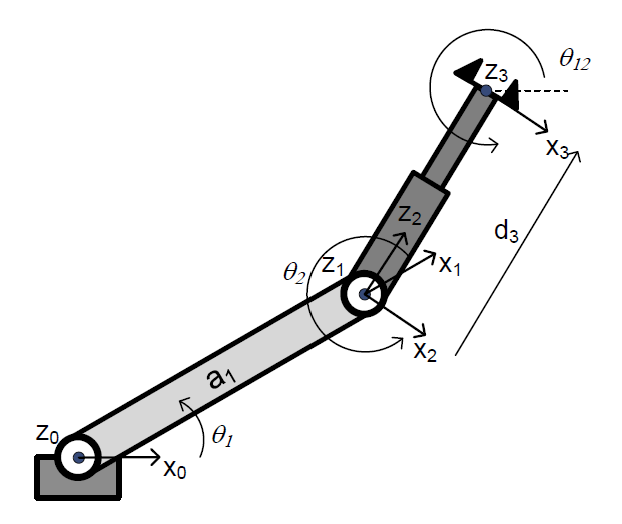
\includegraphics[width=0.5\linewidth]{figs/Q2_PEND.png}
    \end{figure*}

    The rotation matrices and displacements between frames are shown below.

    \centering
    $C_1^0 =
        \begin{bmatrix}
            \cos(\theta_1) & -\sin(\theta_1) & 0 \\
            \sin(\theta_1) & \cos(\theta_1)  & 0 \\
            0              & 0               & 1 \\
        \end{bmatrix}
    $,
    $\vec{r}^{\;0}_{01} =
        \begin{bmatrix}
            a_1\cos(\theta_1) \\
            a_1\sin(\theta_1) \\
            0                 \\
        \end{bmatrix}
    $,
    $C_2^1 =
        \begin{bmatrix}
            \cos(\theta_2) & 0  & -\sin(\theta_2) \\
            \sin(\theta_2) & 0  & \cos(\theta_2)  \\
            0              & -1 & 0               \\
        \end{bmatrix}
    $

    \qquad \qquad \qquad \qquad \quad
    $\vec{r}^{\;1}_{12} =
        \begin{bmatrix}
            0 \\
            0 \\
            0 \\
        \end{bmatrix}$,
    $C_3^2 =
        \begin{bmatrix}
            1 & 0 & 0  \\
            0 & 0 & -1 \\
            0 & 1 & 0  \\
        \end{bmatrix}
    $,\quad
    $\vec{r}^{\;2}_{23} =
        \begin{bmatrix}
            0   \\
            0   \\
            d_3 \\
        \end{bmatrix}
    $
}

\begin{parts}
    \part{Determine the rotation matrix $C_3^0$.}

    \solution
    $C_3^0$ can be determined by the following series of matrix multiplications.

    \begin{equation}
        \begin{split}
            C_3^0 & = C_1^0C_2^1C_3^2
        \end{split}
    \end{equation}

    \begin{equation*}
        \begin{split}
            C_3^0 & =
            \begin{bmatrix}
                \cos(\theta_1) & -\sin(\theta_1) & 0 \\
                \sin(\theta_1) & \cos(\theta_1)  & 0 \\
                0              & 0               & 1 \\
            \end{bmatrix}
            \begin{bmatrix}
                \cos(\theta_2) & 0  & -\sin(\theta_2) \\
                \sin(\theta_2) & 0  & \cos(\theta_2)  \\
                0              & -1 & 0               \\
            \end{bmatrix}
            \begin{bmatrix}
                1 & 0 & 0  \\
                0 & 0 & -1 \\
                0 & 1 & 0  \\
            \end{bmatrix} \\
            C_3^0 & =
            \begin{bmatrix}
                \cos(\theta_1)\cos(\theta_2) - \sin(\theta_1)\sin(\theta_2) & -\cos(\theta_1)\sin(\theta_2) - \cos(\theta_2)\sin(\theta_1) & 0 \\
                \cos(\theta_1)\sin(\theta_2) + \cos(\theta_2)\sin(\theta_1) & \cos(\theta_1)\cos(\theta_2)-\sin(\theta_1)\sin(\theta_2)    & 0 \\
                0                                                           & 0                                                            & 1 \\
            \end{bmatrix}
        \end{split}
    \end{equation*}
    \part{Determine the translation vector $\vec{r}^{\;0}_{03}$}

    \solution
    $\vec{r}^{\;0}_{03}$ by the following summation of transformed relative frame vectors.

    \begin{equation}
        \begin{split}
            \vec{r}^{\;0}_{03} & = \vec{r}^{\;0}_{01} + C_1^0\vec{r}^{\;1}_{12} + C_2^0\vec{r}^{\;2}_{23}
        \end{split}
    \end{equation}

    The second term in this summation is eliminated given $\vec{r}^{\;1}_{12} =
        \begin{bmatrix}
            0 \\
            0 \\
            0 \\
        \end{bmatrix}$. In addition to this, $C_2^0$ is defined as

    \begin{equation*}
        \begin{split}
            C_2^0 & =
            \begin{bmatrix}
                \cos(\theta_1) & -\sin(\theta_1) & 0 \\
                \sin(\theta_1) & \cos(\theta_1)  & 0 \\
                0              & 0               & 1 \\
            \end{bmatrix}
            \begin{bmatrix}
                \cos(\theta_2) & 0  & -\sin(\theta_2) \\
                \sin(\theta_2) & 0  & \cos(\theta_2)  \\
                0              & -1 & 0               \\
            \end{bmatrix} \\
            & =
            \begin{bmatrix}
                \cos(\theta_1)\cos(\theta_2) - \sin(\theta_1)\sin(\theta_2) & 0  & -\cos(\theta_1)\sin(\theta_2) - \cos(\theta_2)\sin(\theta_1) \\
                \cos(\theta_1)\sin(\theta_2) + \cos(\theta_2)\sin(\theta_1) & 0  & \cos(\theta_1)\cos(\theta_2)-\sin(\theta_1)\sin(\theta_2)    \\
                0                                                           & -1 & 0                                                            \\
            \end{bmatrix}
        \end{split}
    \end{equation*}

    The summation becomes the following

    \begin{equation*}
        \begin{split}
            \vec{r}^{\;0}_{03} & =
            \begin{bmatrix}
                a_1\cos(\theta_1) \\
                a_1\sin(\theta_1) \\
                0                 \\
            \end{bmatrix}
            +
            C_2^0
            \begin{bmatrix}
                0   \\
                0   \\
                d_3 \\
            \end{bmatrix} \\
            & =
            \begin{bmatrix}
                a_1\cos(\theta_1)-d_3(\cos(\theta_1)\sin(\theta_2)+\cos(\theta_2)\sin(\theta_1))     \\
                a_1\sin(\theta_1) - d_3(\sin(\theta_1)\sin(\theta_2) - \cos(\theta_1)\cos(\theta_2)) \\
                0                                                                                    \\
            \end{bmatrix}
        \end{split}
    \end{equation*}

    \part{Determine the following angular velocities as skew-symmetric matrices $\Omega$ and vectors $\vec{\omega}$. Note $\theta_1$, $\theta_2$, and $d_3$ can vary with time.}
    \begin{subparts}

        \solution
        The following relationship was used to solve these problems:

        \begin{equation}
            \begin{split}
                \dot{C}_b^a & = \Omega^{\;a}_{ab}C_b^a
                \label{eq:cdot}
            \end{split}
        \end{equation}

        This relationship yields the following:

        \begin{equation}
            \begin{split}
                \Omega_{ab}^{\;a}  & = \dot{C}^a_b(C^a_b)^{-1} \\
            \end{split}
            \label{eq:skew}
        \end{equation}

        \subpart{${\Omega}^0_{01}$, $\vec{\omega}^0_{01}$}

        \solution
        $\dot{C}^a_b$ and subsequent $\dot{C}$ were calculated using \codeword{diff()} in MATLAB\@. The following depicts the corresponding solution:

        \begin{equation*}
            \begin{split}
                {\Omega}^0_{01} & = \dot{C}^0_1(C^0_1)^{-1}\\
                & =
                \begin{bmatrix}
                    -\dot{\theta_1}\sin{\theta_1} & -\dot{\theta_1}\cos{\theta_1} & 0 \\
                    \dot{\theta_1}\cos{\theta_1}  & -\dot{\theta_1}\sin{\theta_1} & 0 \\
                    0                             & 0                             & 0 \\
                \end{bmatrix}
                \begin{bmatrix}
                    \cos(\theta_1) & -\sin(\theta_1) & 0 \\
                    \sin(\theta_1) & \cos(\theta_1)  & 0 \\
                    0              & 0               & 1 \\
                \end{bmatrix}^{-1} \\
                & =
                \begin{bmatrix}
                    0              & -\dot{\theta_1} & 0 \\
                    \dot{\theta_1} & 0               & 0 \\
                    0              & 0               & 0 \\
                \end{bmatrix} \\
                \vec{\omega}^0_{01} & =
                \begin{bmatrix}
                    0              \\
                    0              \\
                    \dot{\theta_1} \\
                \end{bmatrix}
            \end{split}
        \end{equation*}


        \subpart{${\Omega}^1_{12}$, $\vec{\omega}^1_{12}$}

        \solution
        \begin{equation*}
            \begin{split}
                {\Omega}^1_{12} & = \dot{C}^1_2(C^1_2)^{-1}\\
                & =
                \begin{bmatrix}
                    -\dot{\theta_2}\sin{\theta_2} & 0 & -\dot{\theta_2}\cos{\theta_2} \\
                    \dot{\theta_2}\cos{\theta_2}  & 0 & -\dot{\theta_2}\sin{\theta_2} \\
                    0                             & 0 & 0                             \\
                \end{bmatrix}
                \begin{bmatrix}
                    \cos(\theta_2) & 0  & -\sin(\theta_2) \\
                    \sin(\theta_2) & 0  & \cos(\theta_2)  \\
                    0              & -1 & 0               \\
                \end{bmatrix}^{-1} \\
                & =
                \begin{bmatrix}
                    0              & -\dot{\theta_2} & 0 \\
                    \dot{\theta_2} & 0               & 0 \\
                    0              & 0               & 0 \\
                \end{bmatrix} \\
                \vec{\omega}^0_{01} & =
                \begin{bmatrix}
                    0              \\
                    0              \\
                    \dot{\theta_2} \\
                \end{bmatrix}
            \end{split}
        \end{equation*}

        \subpart{${\Omega}^2_{23}$, $\vec{\omega}^2_{23}$}

        \solution
        \begin{equation*}
            \begin{split}
                {\Omega}^2_{23} & = \dot{C}^2_3(C^2_3)^{-1}\\
                & =
                \begin{bmatrix}
                    0 & 0 & 0 \\
                    0 & 0 & 0 \\
                    0 & 0 & 0 \\
                \end{bmatrix}
                \begin{bmatrix}
                    1 & 0 & 0  \\
                    0 & 0 & -1 \\
                    0 & 1 & 0  \\
                \end{bmatrix}^{-1} \\
                & =
                \begin{bmatrix}
                    0 & 0 & 0 \\
                    0 & 0 & 0 \\
                    0 & 0 & 0 \\
                \end{bmatrix} \\
                \vec{\omega}^0_{01} & =
                \begin{bmatrix}
                    0 \\
                    0 \\
                    0 \\
                \end{bmatrix}
            \end{split}
        \end{equation*}

        \subpart{${\Omega}^0_{03}$, $\vec{\omega}^0_{03}$}

        \solution
        Like position vectors in~\ref*{part@2@2}, angular velocities in different frames can be transformed and summed to find other relative angular velocities.

        \begin{equation*}
            \begin{split}
                \vec{\omega}^0_{03} & = \vec{\omega}^0_{01} + C_1^0\vec{\omega}^{1}_{12} + C_2^0\vec{\omega}^{\;2}_{23} \\
                & =
                \begin{bmatrix}
                    0              \\
                    0              \\
                    \dot{\theta_1} \\
                \end{bmatrix} +
                \begin{bmatrix}
                    \cos(\theta_1) & -\sin(\theta_1) & 0 \\
                    \sin(\theta_1) & \cos(\theta_1)  & 0 \\
                    0              & 0               & 1 \\
                \end{bmatrix}
                \begin{bmatrix}
                    0              \\
                    0              \\
                    \dot{\theta_2} \\
                \end{bmatrix} + 0 \\
                & =
                \begin{bmatrix}
                    0                 \\
                    0                 \\
                    \theta_1+\theta_2 \\
                \end{bmatrix}
            \end{split}
        \end{equation*}

        Therefore,

        \begin{equation*}
            \begin{split}
                {\Omega}^0_{03} & =
                \begin{bmatrix}
                    0                 & -(\theta_1+\theta_2) & 0 \\
                    \theta_1+\theta_2 & 0                    & 0 \\
                    0                 & 0                    & 0 \\
                \end{bmatrix}
            \end{split}
        \end{equation*}



    \end{subparts}

\end{parts}